\chapter{Bevezetés}
Ebben a dolgozatban a BME VIK Villamosmérnök MSc képzés Önálló Laboratórium 1 c. tárgyának keretében végzett kutatási és tervezési munkámat összegzem. A dolgozatom témája egy kevéssé ismert nyomtatott antennatípus, a BIFA (Balanced Inverted F Antenna) tervezése.
\section{Céges háttér}
A BIFA tervezésének apropója az, hogy a Silicon Laboratories-nél kis méretű, körülbelül 3-szor 5 cm-es ,,radio board''-ok fejlesztésével is foglalkoznak, amelyek referencia implementációként szolgálnak a cég által termelt rádió IC-ket használó áramkörökhöz. Ezek alapján a Silabs ügyfelei (más cégek) már a végfelhasználóknak szánt rádiós eszközöket gyártanak. A radio boardok sokféle változatban készülnek, több frekvenciasávra, különböző rádiós protokollokat támogatnak, stb. Az egyik érintett frekvenciasáv a \SI{2,4}{GHz}-es ISM sáv, ahol például a Bluetooth protokoll is működik. A radio boardoknak többféle elrendezésben is helyt kell állniuk, sokuk egy nagyobb alaplaphoz (WSTK, Wireless Starter Kit Mainboard) csatlakoztatva rádiós kiegészítő kártyaként tud működni, de vannak olyanok is, amelyek önállóan elemről, vagy többféle módon is működtethetőek.
\begin{figure}[h]
	\centering
	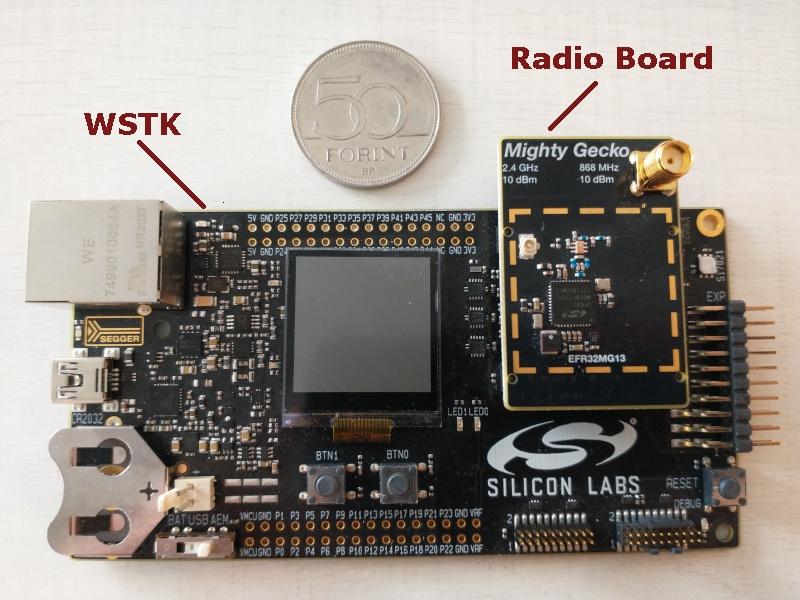
\includegraphics[width=0.6\textwidth]{kep/wstk-rb.jpg}
	\caption{Egy radio board a képen nem kivehető nyomtatott IFA-val egy WSTK-hoz csatlakoztatva.}
	\label{fig:wstk-rb}
\end{figure}
\par A radio boardok többségét WSTK-ra csatlakoztatva fejlesztik és tesztelik, de a végső vezetéknélküli termék már sok esetben a WSTK nélkül kerül felhasználásra. Ráadásul a radio board és a WSTK földkitöltése RF szempontból elég jól össze van kötve a 2 db 40 pines csatlakozó föld-pinjein keresztül, amikkel a két egység csatlakozik egymáshoz, ezért jogos a WSTK-t a monopól antenna szempontjából az alaplap kiterjesztéseként kezelni. Fontos tehát, hogy ne legyen lényeges különbség az antenna működésében a WSTK-t használó és az anélküli elrendezések között, innen az igény egy olyan antennára, ami érzéketlen a WSTK jelenlétére.
\section{Antennák jellemzői, definíciók}
	A különböző antennák összehasonlításának jó eszközei a következő paraméterek, amelyek segítségével több szempontból nyerhetünk betekintést az antennák működésébe.
	\subsection{Iránykarakterisztika, irányhatás és nyereség}
		\par Az antennák alapvető célja, hogy messzire jutó elektromágneses hullámokat hozzanak létre. A létrehozott hullámok energiát szállítanak, teljesítmény áramlik belőlük a szabad térbe. A sugárzási tulajdonságok leírásához gömbi koordinátarendszert $(r, \theta, \phi)$ szokás használni. Az antenna (teljesítmény-) iránykarakterisztikája ($G(\theta, \phi)$) azt írja le, hogy egy az antenna körüli, megfelelően nagy $r$ sugarú gömb felületén hogyan oszlik el az antenna bemenetén betáplált teljesítmény. A nyereség képlete \aref{equ:G}. egyenletben látható, ahol $S(r,\theta,\phi)$ a gömbi koordinátákkal megadott pontban az antenna által létrehozott felületi teljesítménysűrűség, $P_{be}$ az antennába betáplált teljesítmény, $S_0$ pedig az ideális izotróp antenna által létrehozott felületi teljesítménysűrűség azonos $r$ távolságban.
		\begin{align}
			\begin{split}
				\label{equ:G}
				G(\theta,\phi) & = \frac{S(r,\theta,\phi)}{S_0}\\
				S_0 & = \frac{P_{be}}{4\pi r^2}
			\end{split}
		\end{align}
		\par Az iránykarakterisztika értéke egy adott $(\theta, \phi)$ irányban, az ahhoz az irányhoz tartozó nyereség. A szakirodalomban a nyereség kifejezés alatt legtöbbször az iránykarakterisztika maximumát kell érteni, ezt hol $G_{max}$-szal, hol egyszerűen $G$-vel jelölik ezt és általában nem viszonyszámban, hanem dB-ben adják meg. A továbbiakban $G$-vel jelölöm a nyereség dB-ben kifejezett értékét.
		\par Az irányhatás a nyereséghez nagyon hasonló mennyiség, a kettő között az egyedüli különbség, hogy a $P_{be}$ összes betáplált teljesítmény helyett az irányhatás esetében $P_{s}$ összes kisugárzott teljesítmény szerepel.
		\begin{align}
			\begin{split}\label{equ:D}
				D & = \frac{S(r,\theta,\phi)}{S_0'}\\
				S_0' & = \frac{P_s}{4\pi r^2}
			\end{split}
		\end{align}
		\par Ez azt jelenti, hogy a nyereségnél figyelembe vesszük az antenna veszteségeit, míg az irányhatásnál nem.
		\subsection{Hatásfok}
			A fent említett kapcsolatot az antenna nyeresége és irányhatása között a hatásfok ($\eta$) teremti meg. Ezt a szokásos módon definiáljuk \aref{equ:eta}. egyenlet szerint. A hatásfokot viszonyszámban, \%-ban vagy dB-ben szokás megadni, a dB egység előnye, hogy ekkor a szintén dB-ben kifejezett nyereség és irányhatás különbsége a hatásfok.
		\begin{align}
			\begin{split}\label{equ:eta}
				\eta & = \frac{P_{be}}{P_s} \\
				\eta & = G - D \quad [\text{dB}]
			\end{split}
		\end{align}
		\subsection{Antenna $Q$}
		A $Q$ paraméter eredetileg diszkrét reaktáns alkatrészek jellemzésére lett bevezetve (tekercs, kondenzátor, rezgőkörök, stb.) \cite{story-of-q}. Míg reaktáns alkatrészeknél (tekercs, kondenzátor, rezonátorok, stb.) a nagyobb $Q$ jelent jobb minőségű alkatrészt (innen a $Q$ gyakran használatos ,, Quality factor'' feloldása), antennáknál a $Q$ csökkentésére szoktunk törekedni. A $Q$ egyik képlete \aref{equ:Q}. egyenletben látható \cite{multi-band}.
		\begin{align}
			\begin{split}\label{equ:Q}
				Q_1 & = \omega \cdot \frac{\text{térben tárolt maximális energia}}{\text{átlagos veszteségi teljesítmény}} = \\
				& = \omega \cdot \frac{E_{E, max}+E_{M, max}}{P_V},
			\end{split}
		\end{align}
		ahol $\omega$ a működési körfrekvencia, $E_E$ és $E_M$ az elektromos-, ill. mágneses térben tárolt energia, $P_V$ pedig az átlagos veszteségi teljesítmény, amibe antenna esetén beleszámít a kisugárzott teljesítmény is a tényleges veszteség mellett. Ezutóbbi többnyire vezetési- és dielektromos veszteségből tevődik össze, legtöbbször a mágneses hiszterézisveszteség elhanyagolható. Ha egy antennának nagy a $Q$-ja, akkor ez az antenna a betáplált teljesítménnyel hajlamosabb felépíteni az elektromos és mágneses teret maga körül, mint kisugározni azt. Persze egy idő után a térben tárolt energia állandósul, $P_V$ egyenlő lesz a betáplált teljesítménnyel. A tényleges veszteségek a tárolt energia növekedésével nőnek, ezért a nagy $Q$-jú antennák általában kisebb hatékonyságúak, a betáplált hasznos teljesítményt kisebb részét sugározzák ki. Antennáknál a nagy $Q$ egy másik negatív hatása a sávszélesség csökkenése, sok esetben pedig szélessávú antennákat igyekszünk készíteni, emiatt is indokolt a $Q$ csökkentésére való törekvés.
		\par A $Q$-t egy alternatív definícióval is szokás használni rezonátorok esetén, ennek képlete \aref{equ:Q2}. egyenletben látható.
		\begin{align}
			\begin{split}\label{equ:Q2}
				Q_2 & = \frac{f_0}{\Delta f},
			\end{split}
		\end{align}
		ahol $f_0$ a rezonanciafrekvencia, $\Delta f$ pedig annak a két frekvenciának a különbsége $f_0$ két oldalán, amiken a rezonátorban maximálisan tárolt energia éppen a fele a rezonanciafrekvencián maximálisan tárolt energiának (3 dB sávszélesség). Röviden a második definíció szerint $Q$ egy rezonátor relatív sávszélességének a reciproka. A helyzetet tovább bonyolítja, hogy a két különböző definícióból adódó $Q$-k értéke közel van egymáshoz, de nem megegyező.
		\begin{align}
			\begin{split}
				Q_1 & \approx Q_2 \\
				Q_1 & \neq Q_2
			\end{split}
		\end{align}
		\par Egy antenna $Q$-ját nem lehet ügyes tervezéssel minden határon túl csökkenteni, mivel az antenna működési hullámhosszra normált mérete meghatároz egy elméleti minimumot a $Q$-jára vonatkozóan. Az antenna méretét egy olyan gömbbel szokás megadni, amiben még éppen elfér az antenna. Ennek a gömbnek a hullámhosszra normált $a$ sugarából szokás kifejezni a $Q$ alsó határát. Ez a téma az elmúlt évtizedekben az antennákkal kapcsolatos elméleti vizsgálódások egy lényeges pontja volt ehhez hozzátartozik egyrészt a minél jobb alsó becslések, másrészt az adott térfogatban (adott sugarú gömbben) megvalósítható lehető legkisebb $Q$-jú antenna keresése \cite{msa}.
\section{Monopól antennák}
\par A BIFA antennatípus nem gyakori a szakirodalomban, az irodalomkutatás során csak néhány cikkben vagy application note-ban találkoztam vele \cite{an847, bifa-be, bifa-ma, bifa-ca}. Ez az antennatípus egy variációja az IFA-nak (Inverted F Antenna, \aref{fig:tipikus_ifa}. ábra), ezért az IFA jellegzetességeiből kiindulva érdemes tárgyalni, amihez érdemes megvizsgálni a monopól antennák általános jellemzőit, mivel az IFA is ebbe az antennacsaládba tartozik.
\begin{figure}[h]
	\centering
	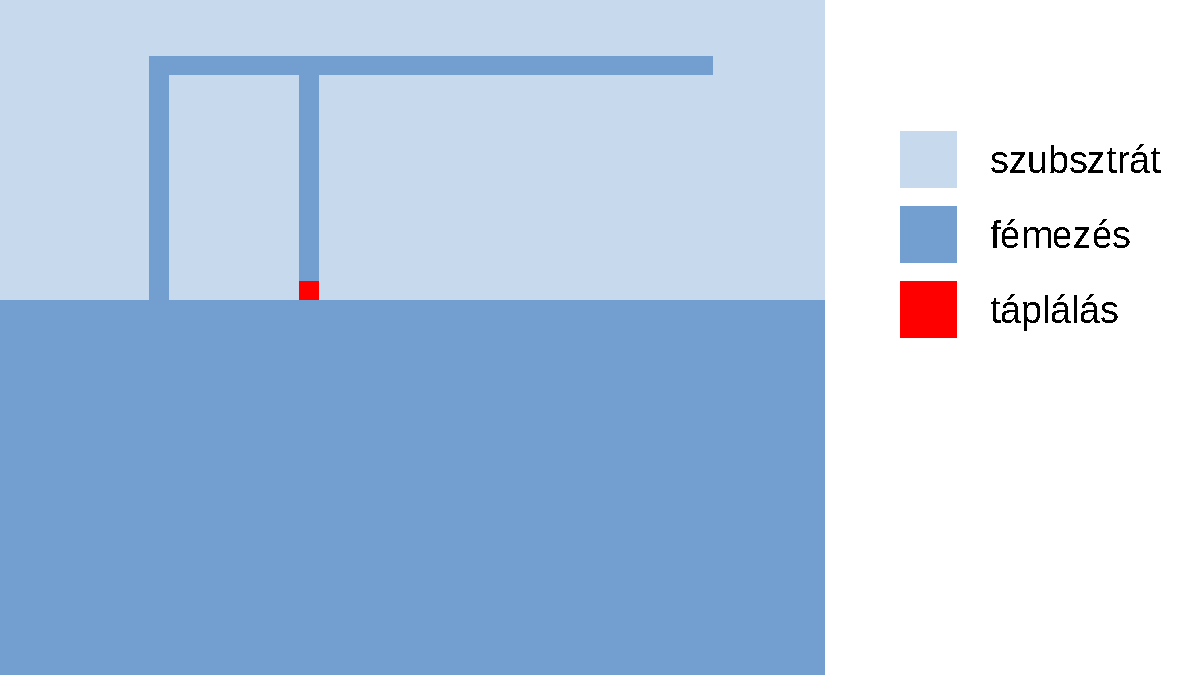
\includegraphics[width=0.6\textwidth]{kep/tipikus_ifa.pdf}
	\caption{Egy tipikus nyomtatott IFA egy nyomtatott áramköri lap szélén.}
	\label{fig:tipikus_ifa}
\end{figure}
\par Az IFA az ILA (Inverted L Antenna) egy variációja (\ref{fig:tipikus_ila}. ábra). Az IFA előnye az ILA-val szemben a megnövekedett abszolút értékű bemeneti impedancia, ami miatt a működési hullámhosszhoz képest kis méretben is jobban használható, könnyebben illeszthető a tápláló hálózathoz. Ezek miatt az IFA-t szélesebb körben alkalmazzák, például mobil eszközökben, ahol az antenna számára rendelkezésre álló hely erősen korlátozott \cite{multi-band}, ekkor bizonyos esetekben a nyomtatott áramköri lapon (NYÁK) kialakított, megfelelő alakú fémezés maga az antenna.
\begin{figure}[h]
	\centering
	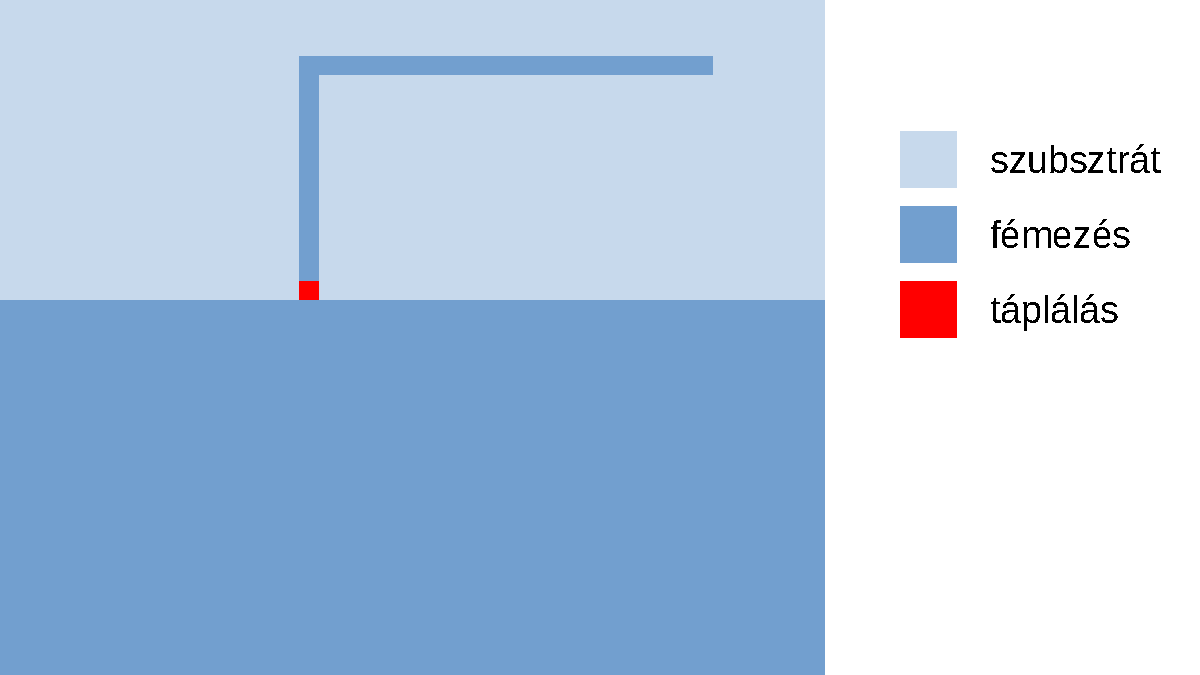
\includegraphics[width=0.6\textwidth]{kep/tipikus_ila.pdf}
	\caption{Egy tipikus ILA egy nyomtatott áramköri lap szélén.}
	\label{fig:tipikus_ila}
\end{figure}
\par A monopól (monopólus) antennákat általában olyankor alkalmazzák, amikor az antenna környezetében egy az antennához képest nagy kiterjedésű vezető található, az ún. alaplap, amit ki lehet használni az antenna sugárzási tulajdonságainak javítására. Ideális esetben az alaplap egy végtelen kiterjedésű és tökéletes elektromos vezető sík. Ekkor a helyettesítő töltések módszerével \cite{fodor} az alaplapot eltávolítva és a monopólt az alaplap síkjára tükrözve egy (a középpontjában a monopóléhoz képest kétszeres feszültséggel gerjesztett) dipól (dipólus) antennát kapunk, amelynek egyik szára az eredeti monopól antenna, ahogy ez \aref{fig:monopol}. ábrán látható.
\begin{figure}[h]
	\centering
	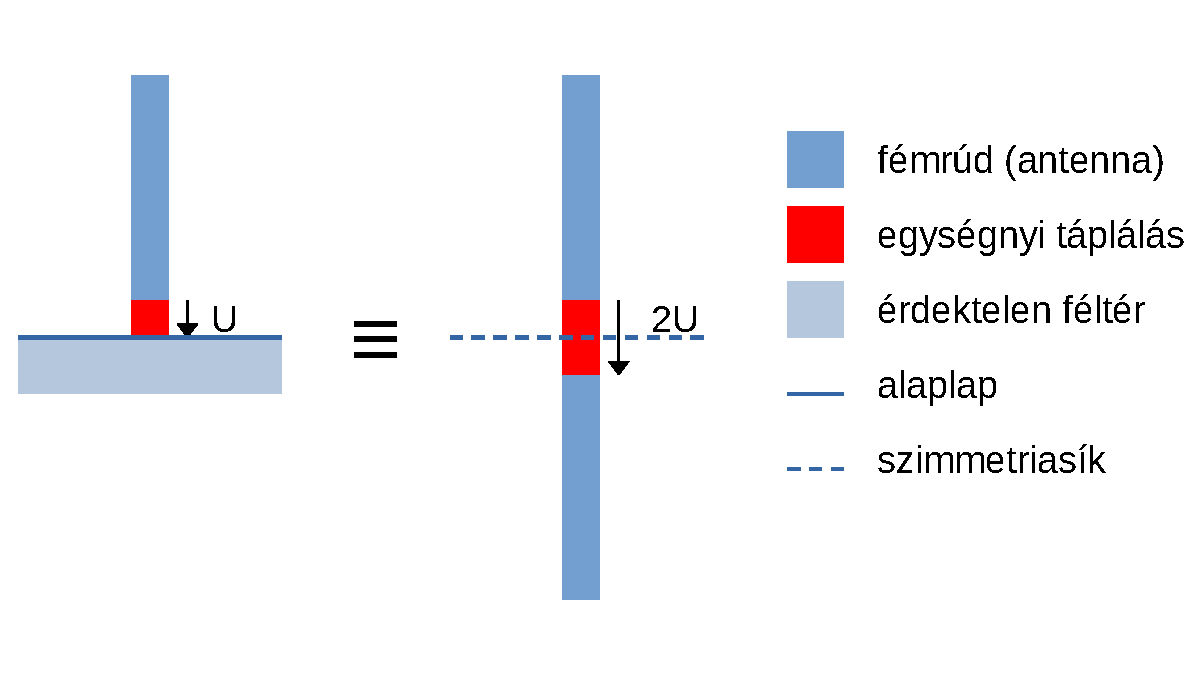
\includegraphics[width=0.6\textwidth]{kep/monopol.pdf}
	\caption{Ideális monopól és ekvivalens dipól.}
	\label{fig:monopol}
\end{figure}
\par Az így kapott antenna az alaplap síkja fölött a monopóluséval megegyező sugárzási karakterisztikát produkál. A monopól esetén az ekvivalens dipól másik szárát az alaplapban indukált áramok hatása helyettesíti, így jön létre a megegyező sugárzási karakterisztika.
\par A fenti helyettesítési módszer nem mindig használható, például egy NYÁK-on kialakított nyomtatott monopól antenna esetén nem, hiszen ekkor legfeljebb a NYÁK földkitöltése tekinthető alaplapnak, de ez messze nem végtelen kiterjedésű, ráadásul az antenna a földkitöltés síkjában helyezkedik el, emiatt nincs értelme a NYÁK síkjára való tükrözésnek. Ehelyett azt a megközelítést érdemes használni a monopól antenna viselkedésének leírásához, ami szerint a nyomtatott antennát és a NYÁK földkiöltését egy erősen aszimmetrikus dipól egy-egy szárának tekintjük \cite{multi-band}.
\par A monopól antennákat használó struktúrák jellemzője, hogy mind az antenna bemeneti impedanciája, mind a sugárzási karakterisztikája érzékeny az alaplap méretének vagy alakjának megváltozására. Ez a jelenség fokozottan jelentkezik akkor, ha az alaplap kis méretű. Ilyen változásokat képes okozni például vezeténélküli mobil eszközöknél, ha a felhasználó a kezébe veszi a készüléket, a fejéhez közel emeli, vagy éppen onnan eltávolítja azt -- mint egy mobiltelefon tipikus használata közben. Az előző példában a felhasználó keze, feje és testének többi része bizonyos keretek között az alaplap kiterjesztésének tekinthető. Emiatt azzal, hogy a kezébe veszi a készüléket, többszörösére növeli az alaplap méretét, ami könnyen okozhat jelentős változásokat az antenna működésében. A változás azonban nem feltétlenül jelent romlást. A modern mobiltelefonok tervezésénél úgy veszik figyelembe a felhasználó kezét, fejét, stb., hogy azok közelségükkel ne rontsák, hanem egyenesen javítsák az antenna tulajdonságait, például megnöveljék a nyereségét, lecsökkentsék a Q-ját és közel izotróp sugárzóvá tegyék azt.
\par A monopól antennák fent vázolt tulajdonságát részben orvosolni lehet, ha differenciális antennával váltjuk ki őket, mert az utóbbi csoportba tartozó antennák jellemzően kevésbé érzékenyek az antennához közeli nagyobb vezető tárgyak elhelyezkedésére. Persze ez sem általánosan igaz, a differenciális antennákra is lehet jelentős hatása a környezet változásának, mint például a reflektort vagy direktort használó antennáknál, amelyek jellemzően érzékenyek a reflektor (direktor) alakjának vagy távolságának változására. A monopól antenna hasonló méretű differenciálisra való cserélésével az antenna effektív mérete könnyen csökkenhet, ahogy \aref{fig:se-diff}. ábrán látható, ezáltal megnőhet a $Q$-ja és lecsökkenhet a sávszélessége.
\begin{figure}[h]
	\centering
	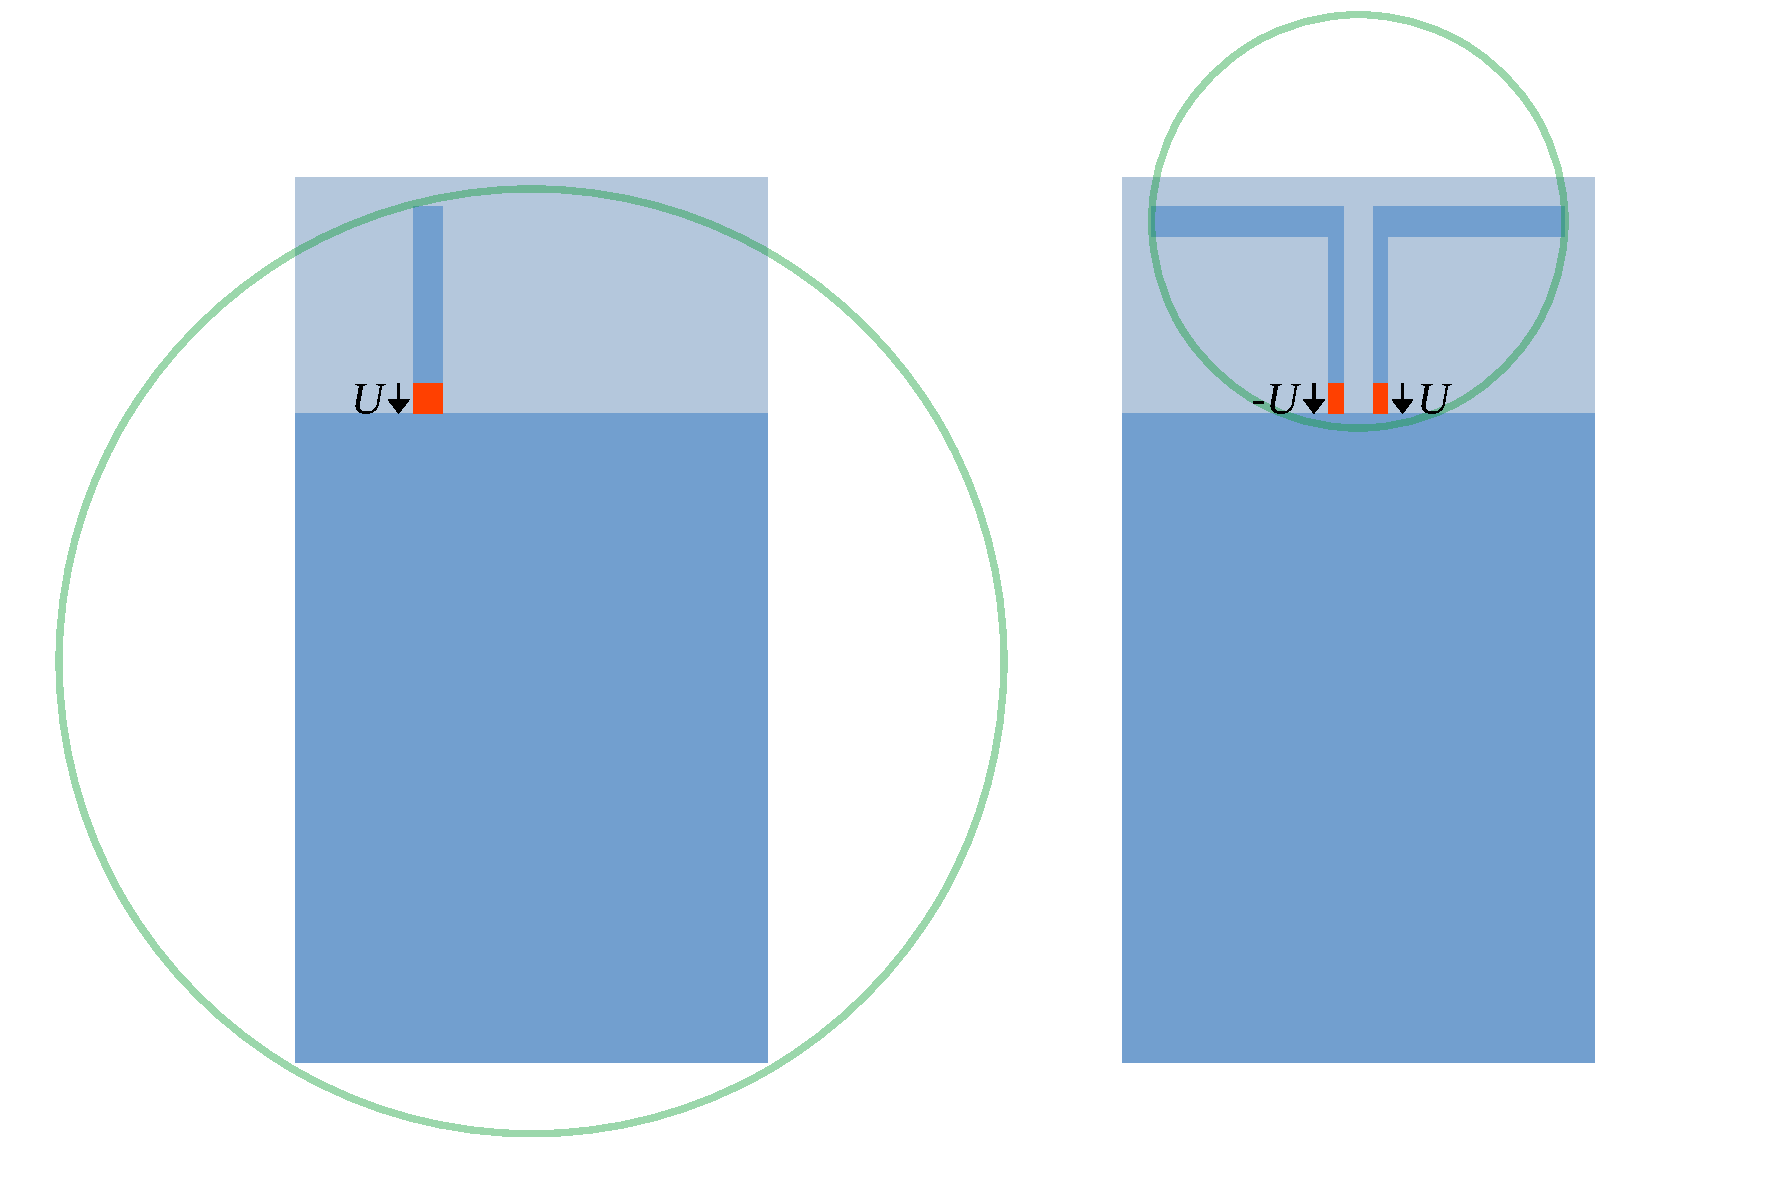
\includegraphics[width=0.8\textwidth]{kep/se-diff.pdf}
	\caption{Monopól antenna diferenciálisra való cserélésével csökken az antenna effektív mérete és csökken a NYÁK hatása a sugárzásra.}
	\label{fig:se-diff}
\end{figure}
\par BIFA-t IFA-ból \aref{fig:ifa-bifa}. ábra szerint lehet megkapni, a differenciális táplálású BIFA a szimmetriasíkja mentén két IFA-ra vágható szét. A tükrözés miatt az ekvivalens fél-BIFA (egy IFA) bemeneti impedanciája éppen a fele a BIFA-nak, mert a bemeneti áram nem változik a két elrendezés között, a beeneti feszültség viszont megduplázódik.
\begin{figure}[h]
	\centering
	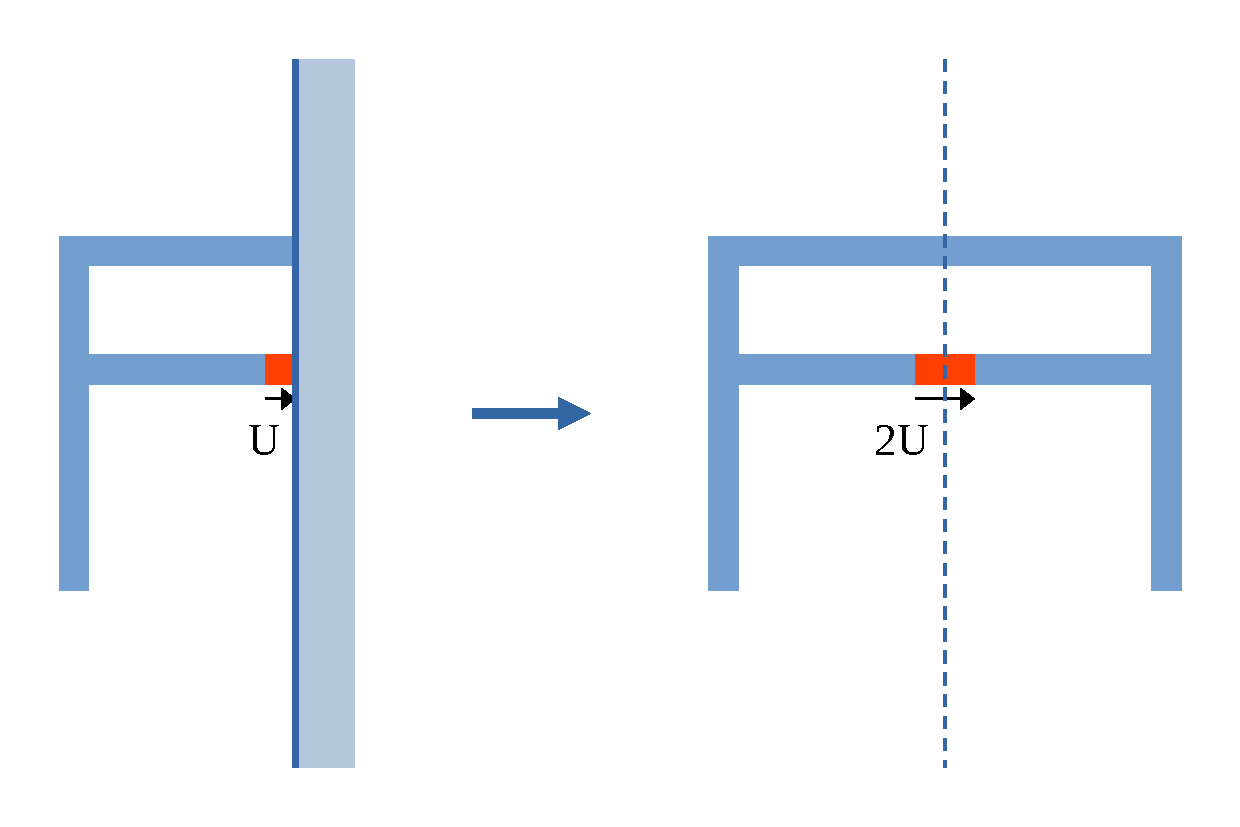
\includegraphics[width=0.6\textwidth]{kep/ifa-bifa.pdf}
	\caption{A BIFA és az IFA kapcsolata.}
	\label{fig:ifa-bifa}
\end{figure}